\section{Metodyka rozwiązania}
\label{sec:metodyka-rozwiazania}
W tej części opisane są szczegółowo metody rozwiązania postawionego w moim projekcie problemu.

\subsection{NodeMCU framework}
NodeMCU jest to framework bazujący na języku Lua dla modułów ESP8266 \autoref{fig:esp-12}.
\begin{figure}[!htbp]
	\centering
	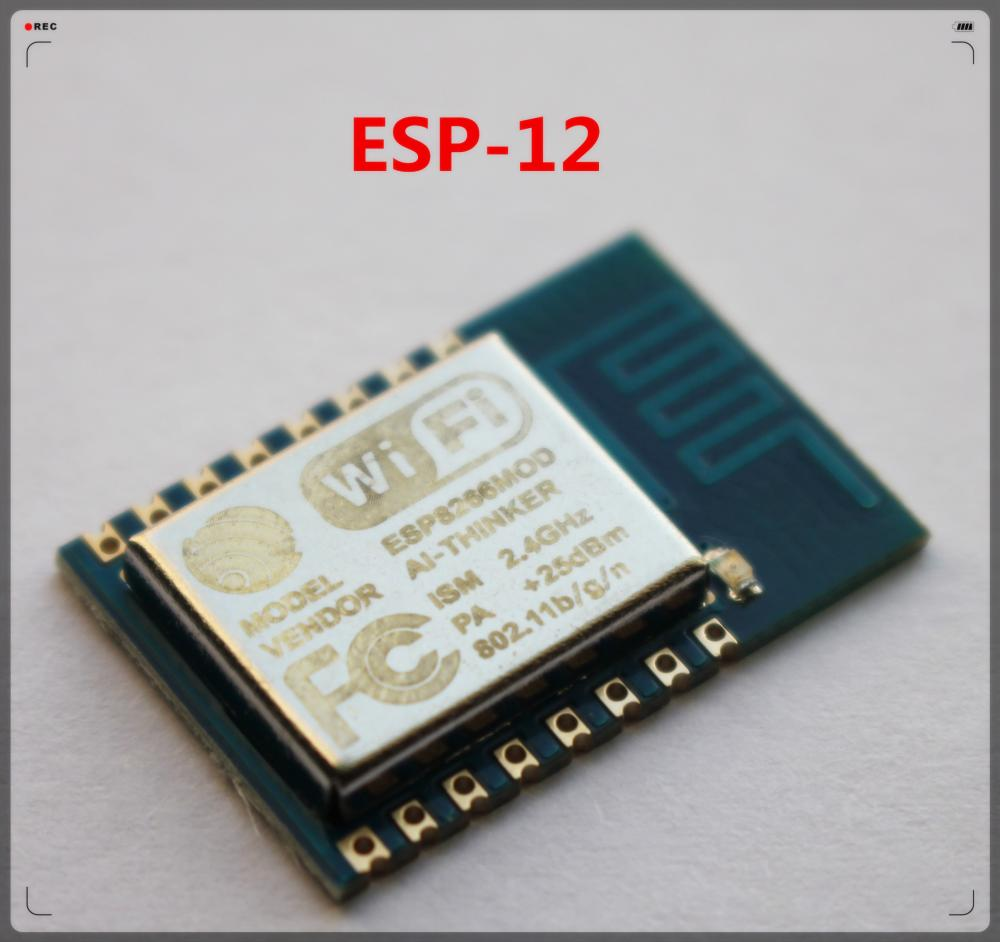
\includegraphics[width=0.7\textwidth]{images/esp-12.jpg}
	\caption[Moduł ESP8266 w wersji 12.]{Moduł ESP8266 w wersji 12} 
	\label{fig:esp-12}
\end{figure}
Znacznie ułatwia on programowanie tych urządzeń, wynika to z kilku faktów:
\begin{itemize}
	\item język Lua jest językiem interpretowanym 
	\item NodeMCU wspiera wiele formatów komunikacji  
	\item posiada wiele zdefiniowanych protokołów IoT
\end{itemize}
Warto tutaj wspomnieć o kilku istotnych funkcjonalnościach oferowanych przez NodeMCU. W szczególności chciałbym pochylić się nad tymi, które zostały użyte w moim projekcie. 

\subsubsection{ADC Module}
Moduł ADC pozwala na dostęp do przetwornika analogowo-cyfrowego. Na ESP8266 występuje jeden tylko pojedynczy kanał, który jest multipleksowany na napięcie baterii. W zależności od ustawień można odczytać zewnętrzne zasilanie, lub zasilanie systemu. 
Ten program zmienia tryb, po jego wykonaniu, moduł się restartuje
\begin{lstlisting}
-- in you init.lua:
if adc.force_init_mode(adc.INIT_VDD33)
then
  node.restart()
  return -- don't bother continuing, the restart is scheduled
end
\end{lstlisting} 
Aby odczytać napięcie zasilania należy wywołać funkcję:
\begin{lstlisting}
val = adc.read(0)
\end{lstlisting} 
Aby odczytać napięcie systemu należy wywołać funkcję:
\begin{lstlisting}
val = adc.readvdd33()
\end{lstlisting} 

\subsubsection{AM2320 Module}
Ten moduł zapewnia obsługę czujnika temperatury AM2320 poprzez interfejs i2c.
\begin{lstlisting}
am2320.init(1, 2)
rh, t = am2320.read()
print(string.format("RH: %s%%", rh / 10))
print(string.format("Temperature: %s degrees C", t / 10))
\end{lstlisting} 


\subsubsection{bit Module}
Zawiera podstawowe operacje na bitach, przedstawione są w \autoref{fig:bit-module}

\begin{table}[t]
\caption{Lista operacji bitowych w NodeMCU}
\label{fig:bit-module}
\begin{tabular}{|r|l|}
  \hline 
  bit.arshift() & Arithmetic right shift a number equivalent to value >> shift in C\\
  \hline 
  bit.band()  & Bitwise AND, equivalent to val1 \& val2 \& \\
  \hline 
  bit.bit() & Generate a number with a 1 bit (used for mask generation)\\
  \hline 
  bit.bnot() & Bitwise negation, equivalent to `~value in C\\
  \hline 
  bit.bor() & Bitwise OR, equivalent to val1 | val2 | \\
  \hline 
  bit.bxor() & Bitwise XOR, equivalent to val1 ^ val2 ^ \\
  \hline 
  bit.clear() & Clear bits in a number\\
  \hline 
  bit.isclear() & Test if a given bit is cleared\\
  \hline 
  bit.isset() & Test if a given bit is set\\
  \hline 
  bit.lshift() & Left-shift a number, equivalent to value << shift in C\\
  \hline 
  bit.rshift() & Logical right shift a number, equivalent to ( unsigned )value >> shift in C\\
  \hline 
  bit.set() & Set bits in a number\\
  \hline
\end{tabular} 
\end{table}

\subsubsection{CJSON Module}
Pozwala na kodowanie i dekodowanie z/do JSON. Niestety moduł ten posiada dużą wadę, otóż może spowodować out-of-memory error, co prowadzi do zresetowania modułu ESP8266. 
Kodowanie tablicy Lua do JSONa:
\begin{lstlisting}
ok, json = pcall(cjson.encode, {key="value"})
if ok then
  print(json)
else
  print("failed to encode!")
end
\end{lstlisting} 
Dekodowanie JSONa do tablicy Lua:
\begin{lstlisting}
t = cjson.decode('{"key":"value"}')
for k,v in pairs(t) do print(k,v) end
\end{lstlisting} 

\subsubsection{CoAP Module}


\subsection{Rozwiązanie bazujące na standardzie telnet}
Finalnym produktem powinien być stabilny prototyp urządzenia, połączony z modułem ESP8266, posiadający przynajmniej jeden czujnik. Użytkownik powinien mieć możliwość zdalnego starowania tym urządzeniem za pomocą mobilnej aplikacji. System powinien składać się przynajmniej z trzech urządzeń, każde z nich powinno automatycznie łączyć się do sieci Wi-Fi po uruchomieniu. 

Dodatkowo, system powinien oferować wygodny interfejs dostępny dla użytkownika końcowego. Udostępnienie API poprzez sterowanie urządzeniami za pomocą telnetu pozwoli na programowy dostęp do sterowania urządzeń z poziomu dowolnego języka programowania. Powinny również zostać zaimplementowane mechanizmy autentykacji zlecanych operacji. Oprócz dostępu programowego, planowana jest implementacja graficznego interfejsu mobilnego, przeznaczonego dla użytkowników\cite{kukdm-art}.

\begin{figure}[!htbp]
	\centering
	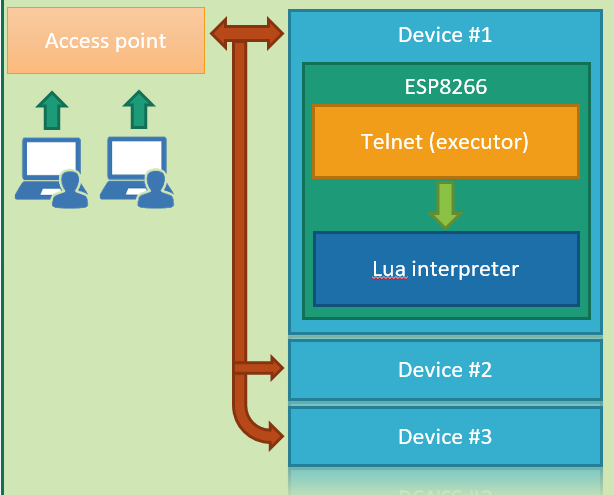
\includegraphics[width=0.9\textwidth]{images/fig01-arch-overview.png}
	\caption[Wizja architektury systemu.]{Wizja miejsca użytkownika, budowy urządzenia, oraz sposobu komunikacji}
	\label{fig:arch-overview}
\end{figure}

Wizję budowy urządzenia przedstawia \autoref{fig:arch-overview}.

\subsection{Rozwiązanie bazujące na CoAP Web Service}

\begin{figure}[!htbp]
	\centering
	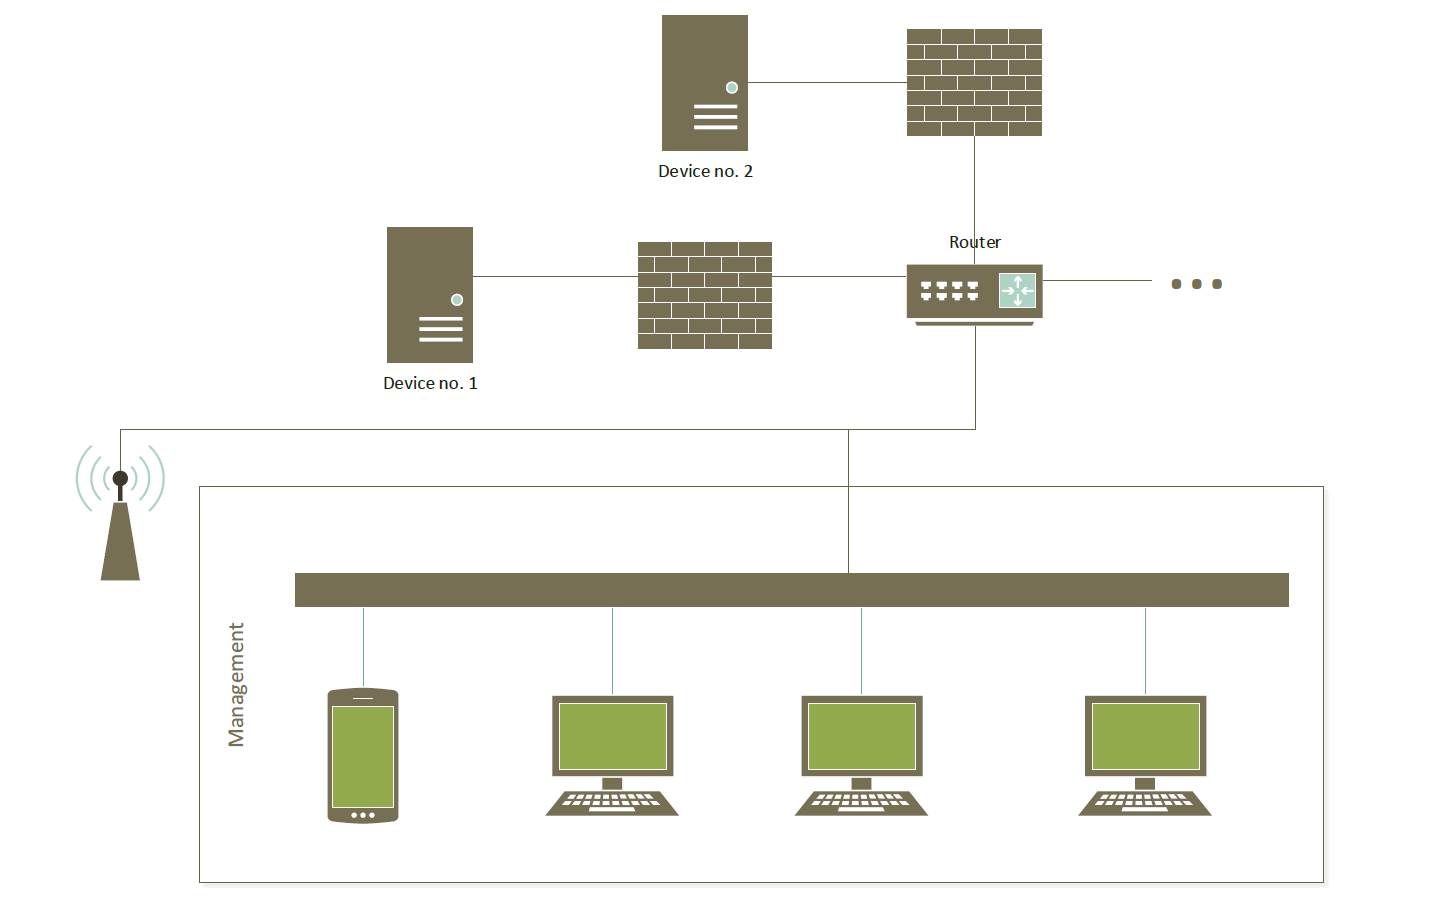
\includegraphics[width=0.9\textwidth]{images/schemat.png}
	\caption[Wizja architektury systemu w standardzie CoAP.]{Wizja miejsca użytkownika, sposobu komunikacji w systemie w standardzie CoAP}
	\label{fig:schemat}
\end{figure}
Wizję budowy urządzenia przedstawia \autoref{fig:schemat}.